% !TEX encoding = UTF-8 Unicode

\section{Les supercalculateurs}\label{sec:supercomputer}
%%%%%%%%%%%%%%%%%%%%%%%%%%%%%%%%%%%%%%%%%%%%%%%%%%%%%%%%%%%%%%%%%
 
Dans la section précédente, nous avons présenté les principales applications utilisées dans le HPC. Ces codes, doivent être exécutés sur des architectures très puissantes pour pouvoir donner des résultats dans des temps raisonnables. Les besoins des applications peuvent être différents. Il peut s'agir d'un besoin de puissance de calcul, de mémoire, de stockage ou de communication. L'infrastructure alors mis en place doit répondre à ces besoins.  


\subsection{Définition et historique}
%%%%%%%%%%%%%%%%%%%%%%%%%%%%%%%%%%%%%%%%

    Pour obtenir une grandes puissance de calculs il est nécessaire de regrouper de centaines (voire de milliers) de ressources qui pour former une grappe de serveurs (cluster). L'infrastructure matériel et logiciel qui résulte du regroupement de serveurs de calculs est appelé un supercalculateur. Celle ci s'occupe alors de la gestion des communications entre les ressources (coeurs de calcul, processeurs, serveurs), l'accès aux donnés simultané ou la tolérance aux fautes. 
    
    Les premiers supercalculateurs étaient des architectures uniques ne pouvant pas être répliqués facilement. On considère que le premier supercalculateur est le CDC6600, en parti élaboré par Seymour Cray, alors employé de l'entreprise Control Data. Il était alors l'ordinateur le plus puissant de la planète grâce à une mémoire de 131000 mots de 60 bits, une fréquence de 40 Mhz et sa capacité calculatoire de $3.3 \times 10^6$ opérations par seconde. A titre de comparaison l'ordinateur portable utilisé pour écrire ce manuscrit est capable d'exécuter plus de $10^9$ opérations par seconde. 
        
    La puissance des processeurs n'a fait qu'évoluer ces trente dernières années. Grâce à l'augmentation de la densité des transistors et de nombreuses évolution technologique, les premiers supercalculateurs monolithiques ont pu être construit. L'augmentation de la vitesse des circuits ainsi que l'augmentation exponentielle du nombre de transistors des circuits à rendu ces systèmes impossible à alimenter en énergie ou à être refroidi. Il a alors fallut repenser l'architecture des supercalculateurs pour continuer à produire des plateformes toujours plus puissantes. Pour continuer à profiter de la loi de Moore et des différentes évolutions technologiques (mémoires, stockage), un nouveau modèle d'infrastructure est alors apparu consistant à agglomérer ces ordinateurs entre eux pour construire une structure plus puissante. On appelle cette infrastructure une grappe (ou \textit{cluster}). L'Intel Paragon est un des premiers exemples de cluster construit par Intel en 1992\footnotetext{source: \url{https://www.top500.org/featured/systems/intel-xps-140-paragon-sandia-national-labs/\#Historical}}, qui regroupe 3680 processeurs indépendant atteignant une puissance regroupé de $143.40 \times 10^9$ flop. Les processeurs alors utilisés sont des microarchitectures spécialisées pour le calcul scientifique, différentes de celles utilisées pour les processeurs grands publique. Aujourd'hui, un supercalculateur moderne est construit avec du matériel produit en série (\textit{commodity hardware}). Que ce soit des processeurs ou de la mémoire, on peut trouver ces matériels sur le marché grand public. C'est seulement l'agglomération de ces milliers de serveurs qui en fait des infrastructures très puissantes. 
    

    \begin{figure}
        \center
        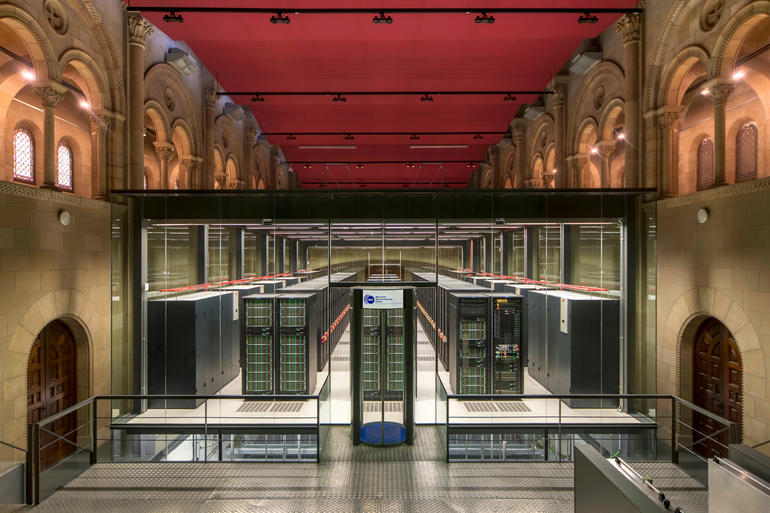
\includegraphics[width=10cm]{images/hpc_bsc_super.jpg}
        \caption{\label{fig:hpc_bsc_super} Le supercalculateur du Centre de Calcul de Barcelone (BSC) est installé dans une ancienne chapelle.}
    \end{figure}

    

\subsection{Architecture des supercalculateurs}
%%%%%%%%%%%%%%%%%%%%%%%%%%%%%%%%%%%%%%%%%%%%%%

\begin{fancyquotes}
Un cluster (grappe) de serveurs est un \textbf{interconnexion} de \textbf{ressources informatiques} dans le but de \textbf{résoudre un problème} complexe de façon \textbf{partagée}. 
\end{fancyquotes}

    L'architecture des supercalculateurs modernes n'est pas très différentes de celle des ordinateurs classiques. La puissance d'une telle plateforme vient seulement de l'agrégation de centaines de ressources de calculs, capables de travailler ensemble pour résoudre un problème complexe. Nous retrouvons dans ces architectures la majorité des composants d'un ordinateur classique. Le domaine du HPC est le domaine informatique qui consiste à exécuter des applications le plus efficacement possible sur de tels architectures. 
    
    Les deux principales caractéristiques d'un supercalculateur sont sa capacité à calculer rapidement ainsi que sa capacité à mémoriser les informations et les résultats produits. Pour cela, l'infrastructure utilisée doit gérer l'équilibrage de la charge de calculs sur les différentes ressources disponibles, la gestion des communications entre les ressources (coeurs de calcul, processeurs, serveurs), l'accès aux données simultané ou encore la tolérance aux fautes. 

    \subsubsection{Les serveurs}
    %%%%%%%%%%%%%%%%%%%%%%%%%%%%%%%%%
        Les serveurs qui sont utilisés dans un supercalculateur possèdent un ou plusieurs processeurs. Comme un ordinateur classique, chaque processeur est relié à la mémoire et au stockage (voir \autoref{fig:motherboard}). En fonction des configurations, chaque serveurs peut être agrémenté d'un ou plusieurs accélérateur (GPU). La principale différence avec un ordinateur classique, autre que la puissance des matériels utilisés, vient du système d'interconnexion (voir \autoref{fig:dl360_back}). Les serveurs doivent pouvoir échanger des informations pour se synchroniser ou partager des résultats entre eux et accéder aux stockage (voir \autoref{sec:edl_interco}).
        
        
        
        \begin{figure}[t!]
            \centering
            \begin{subfigure}[t]{0.48\textwidth}
                \centering
                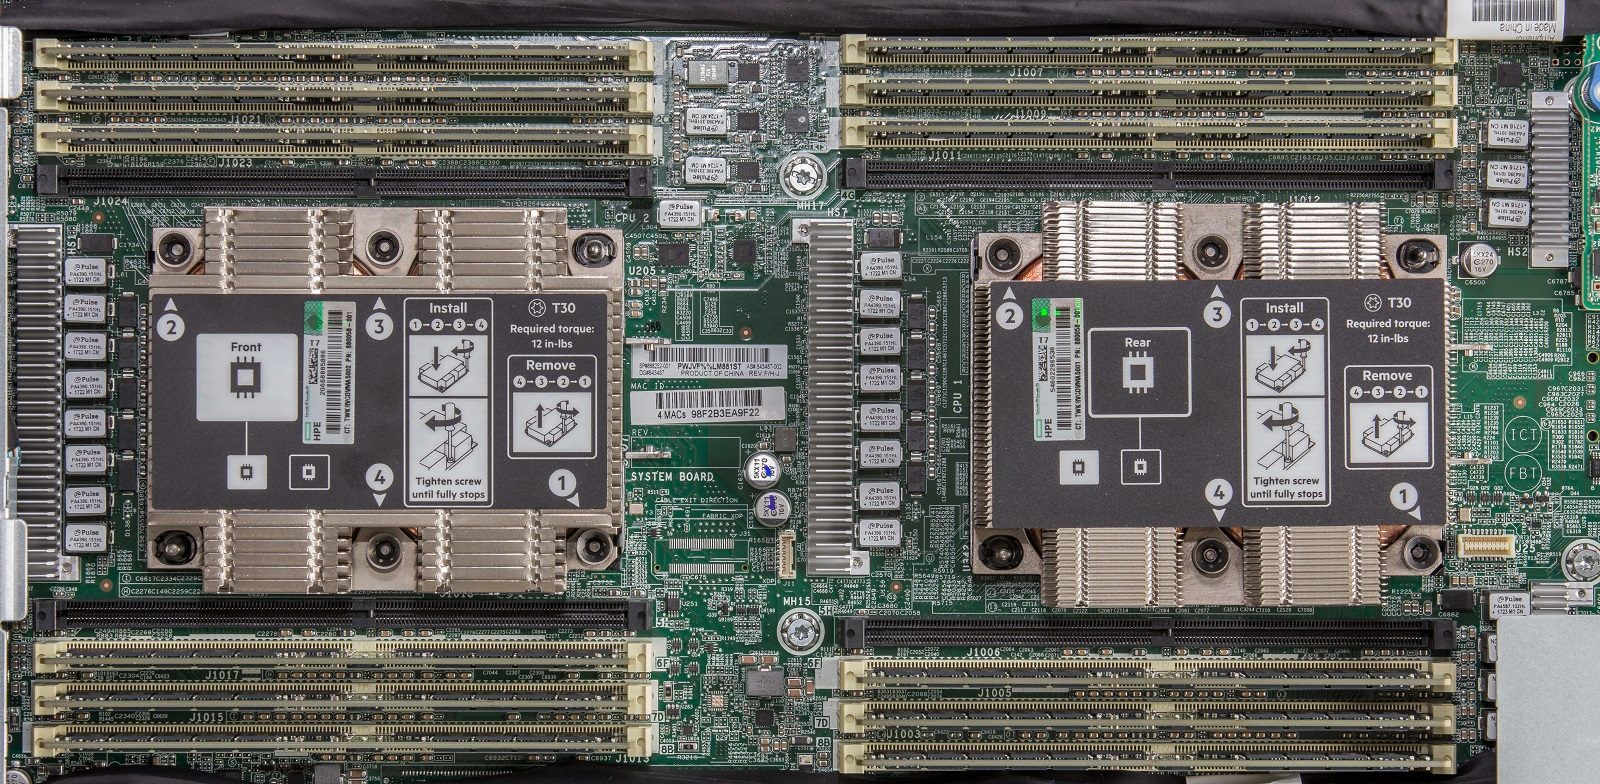
\includegraphics[width=.9\linewidth]{images/motherboard.jpg}
                \caption{\label{fig:motherboard}Carte mère d'un serveur possédant deux processeurs.}
            \end{subfigure}\hfill
        \begin{subfigure}[t]{0.48\textwidth}
                \centering
                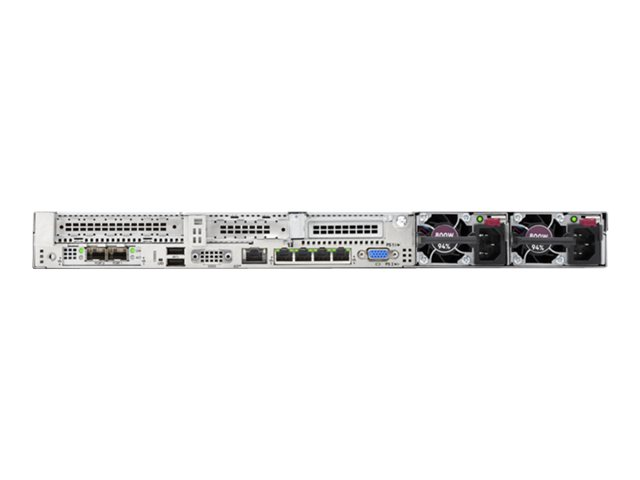
\includegraphics[width=\linewidth]{images/dl360_back.jpg}
                \caption{Vu arrière d'un serveur exposant les différentes interfaces de connexion.\label{fig:dl360_back}}
            \end{subfigure}
            \caption{Exemple d'un serveur utilisé dans les supercalculateur.}
            \label{pic_pi_rect}
        \end{figure}
        
        
        \subsubsection{Les accélérateurs}
        %%%%%%%%%%%%%%%%%%%%%%%%%%%%%%%%%%%%%%%%%%%%%%%%%%%%%%%%%
            Un des principes fondamentale des processeurs énoncé par Von Neumann était leur universalité. Leur faculté à exécuter tout type de code est à la fois une force mais aussi un de leur plus grande faiblesse. Ils sont très peu efficace, en temps et en énergie, pour résoudre certains types de calculs tels que les traitements de signaux ou d'objets géométriques. Pour ces classes de problèmes, des processeurs spécialisés sont venus s'ajouter au processeur pour les aider. Le plus connus et le plus utilisé est le GPU, utilisé pour les calculs graphiques.
            
            Étant architecturalement adapté à certains algorithmes, les accélérateurs sont généralement plus efficace énergétiquement. Dans un contexte où l'énergie est une pression majeure, leur utilisation est d'autant plus pertinente.
             
            Pour pouvoir être utilisé et obtenir les meilleurs performances, les applications doivent être adapté. Cela impose aux développeurs d'apporter des transformations à leur code, d'utiliser un nouveau compilateur ou même un autre langage. Ces transformations peuvent réduire la portabilité de l'application, notamment quand un langage propriétaire, tel que \verb|CUDA| est utilisé.
            
            Un accélérateur peut être adapté à la résolution d'une partie de l'application mais peut être très inefficace pour le reste. Cela rend le choix de l'accélérateur difficile, car l'investissement (budget et modification de code) doit être rentable pour l'utilisateur.

    
        \paragraph{GPU} Les GPU sont les accélérateurs les plus répandus dans les supercalculateur. À l'origine, les GPU étaient destinés à jeux vidéos et aux calculs de rendu graphique. Suite à leur utilisation pour d'autres applications que le rendu graphique, ces accélérateurs sont aussi nommés GP-GPU pour \textit{general purpose GPU}. 
        À l'inverse des processeur les GPU sont composé de nombreux coeurs (plusieurs centaines). Ceux-ci sont moins complexes et performance que les coeurs de processeur, mais leur nombre les rend particulièrement efficace pour certaines application offrant des noyaux de calculs parallélisable. La \autoref{fig:CPUvsGPU} compare l'évolution des performance des GPU avec celles des CPU de même génération. On remarque l'écart significatif séparant leur performance. Cependant, la figure représente la performance théorique des architectures et il est rare que les applications s'en approchent. Cependant, pour des applications particulièrement adaptée, le GPU n'a pas d'équivalent actuellement en terme de performance. La performance du bus mémoire d'un GPU est elle aussi bien supérieur, rendant ces architectures d'autant plus intéressante pour les codes dont la performance est limité par le système mémoire. 
        
        Actuellement, il existe deux fournisseurs principaux de GPU (NVIDIA et AMD) qui ont pu bénéficier de leur longue expérience dans le domaine du jeux vidéo. La première nécessite l'utilisation de langage propriétaire (\verb|CUDA|) quand la deuxième peut être programmée grâce au langage \verb|OpenCL|. Le principale avantage de \verb|CUDA| est de pouvoir utiliser des librairies optimisées par NVIDIA pour ses plateformes pour différents domaines (algèbre linéaire (cuBLAS, CUSPARSE), analyse de signal (cuFFT), apprentissage machine (cuDNN, TensorFlow)). 
        
        \verb|OpenCL| a été initié par Apple et est maintenant maintenu par le groupe Khronos. C'est un standard ouvert et libre de droits permettant l'exécution de codes sur différentes plateformes. Une application utilisant \verb|OpenCL| pourra être, en théorie, facilement portée sur d'autres architectures (CPU, FPGA, DSP). 

        Acutellement, le développement ou le portage d'applications pour pouvoir être exécutées sur ces architectures demande un investissement conséquent. L'architecture spécifique des GPU nécessite au programmeur de présenter explicitement la parallélisation d'un noyau. De plus, le GPU possédant son propre espace mémoire, le programmeur doit gérer explicitement les transferts entre celle-ci et la mémoire centrale du serveur.
        De nombreux travaux essaient de combler cette difficulté. La plus notable étant surement OpenACC. Crée en 2011, cet outil permet d'annoter le code source d'une application à l'aide de \verb|#pragma| pour indiquer au compilateur les zones parallélisable. Avec un effort raisonable, des performances proches des performances atteinte en utilisant \verb|CUDA| peuvent être atteinte. 
        
            \begin{figure}
            \center
            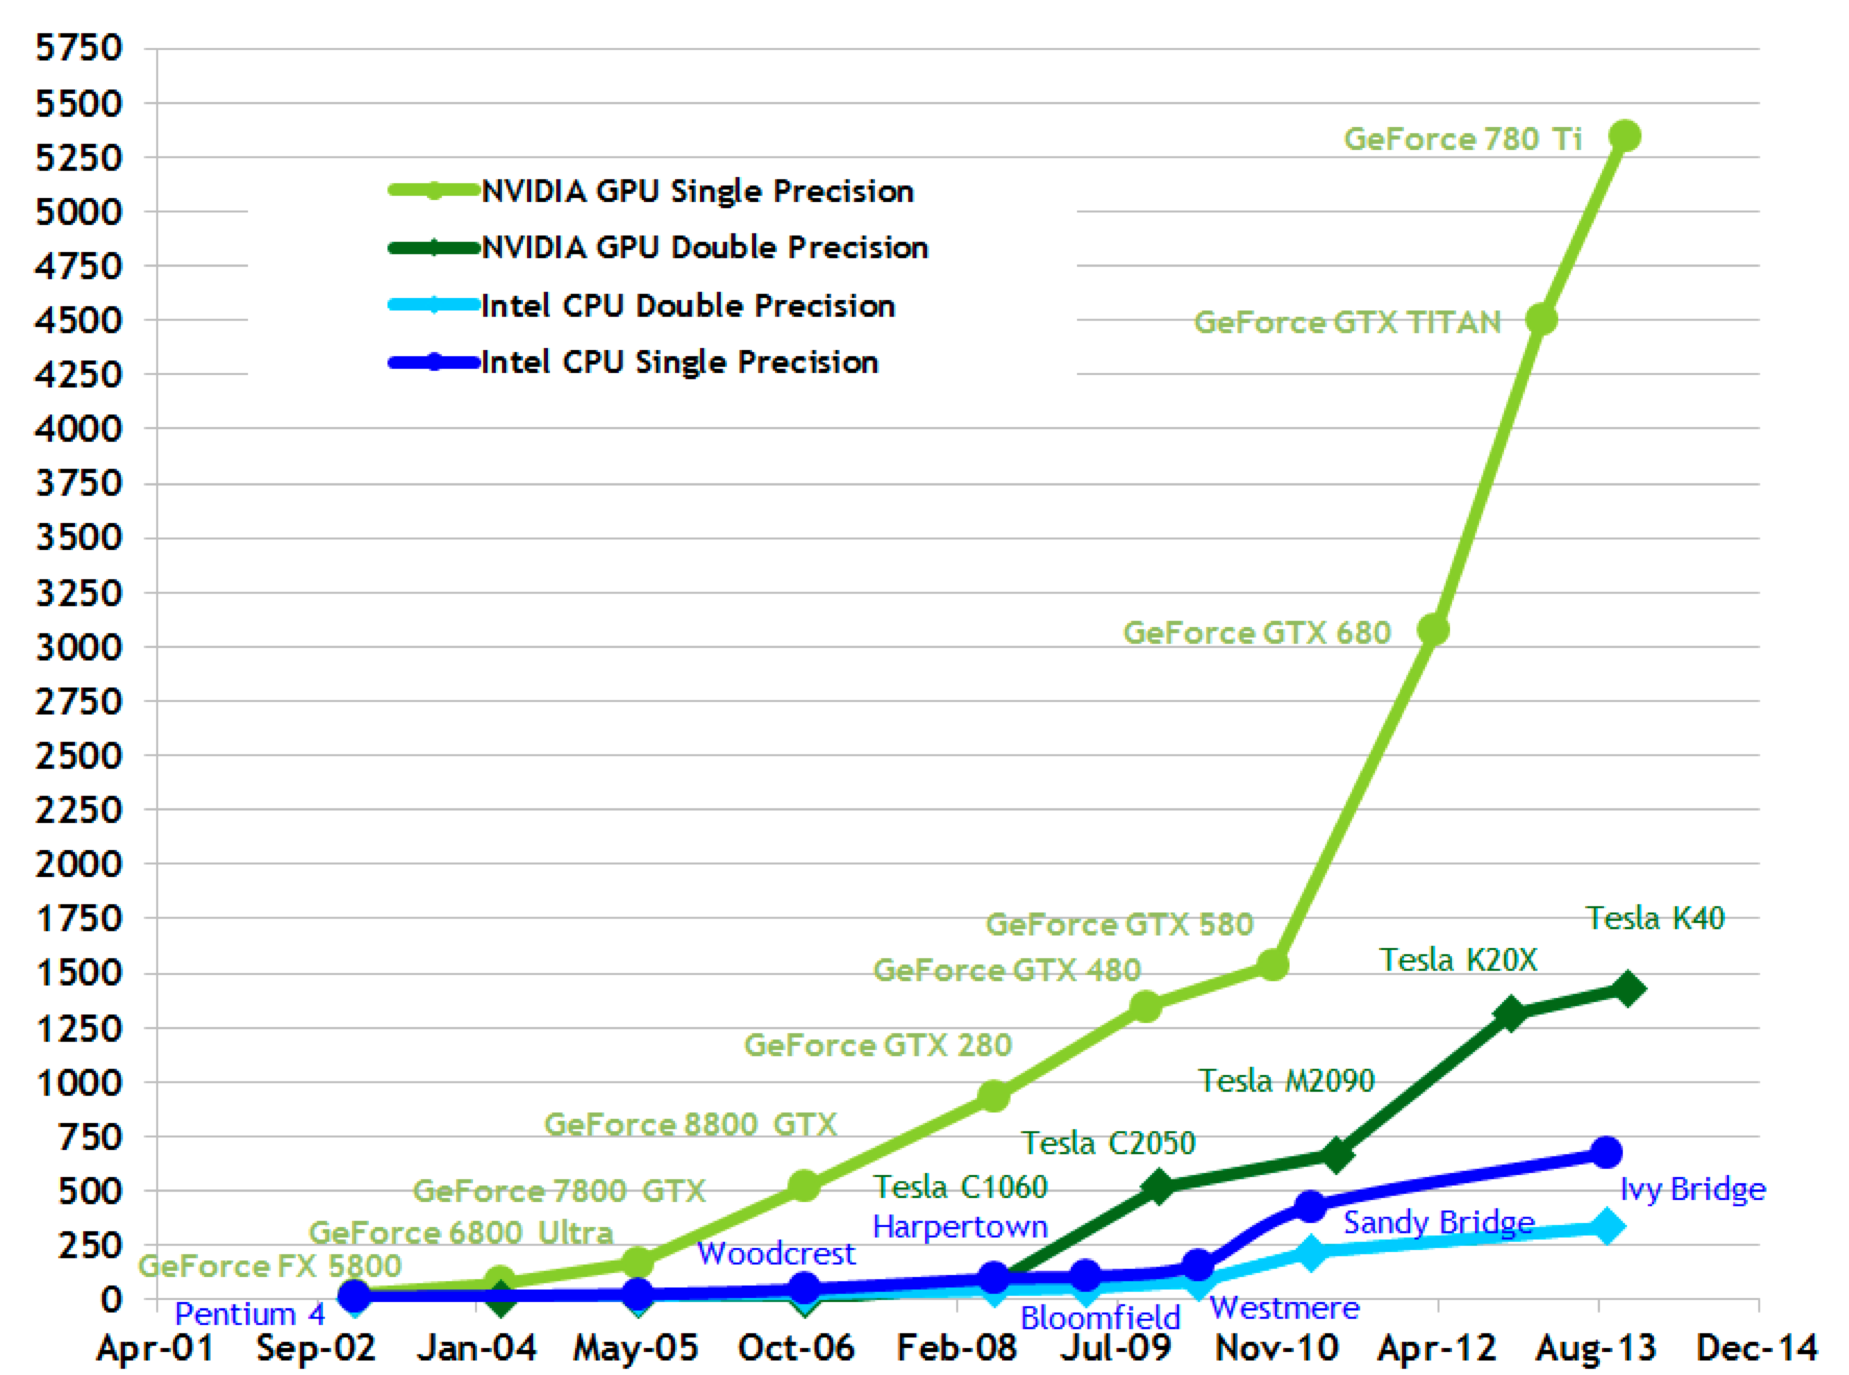
\includegraphics[width=10cm]{images/CPUvsGPU.png}
            \caption{\label{fig:CPUvsGPU} Comparaison des performances entre différentes générations de CPU et GPU}
        \end{figure}
            

        \paragraph{FPGA \textit{Field Programmable Gate Array}).}  Comme l'indique leur nom, les FPGA sont de simples circuits intégrés qui contiennent des portes logiques pouvant être programmé pour la réalisation d'un circuit. 
        Les méthodes traditionnelles de développement sur FPGA nécessitent la conception d'une architecture matérielle utilisant un Hardware Description Language (HDL). Pour ce faire, le développeur doit concevoir les chemins de données, la logique de contrôle, l'interface avec les coeurs matériels de propriété intellectuelle (PI). Il s'agit d'un processus de développement fastidieux et complexe qui peut entraver leur adoption dans de nombreuses applications pratiques. Les FPGA les plus récents peuvent être programmé à l'aide d'\verb|OpenCL|.
        Implémenter un un circuit à l'aide d'un FPGA peut fournir la même efficacité énergétique et la même performance qu'un implémentation ASIC. Cependant, le fait que les FPGA soient programmables leur donne un avantage sur les ASIC, car le même matériel peut être reprogrammé en un nouveau circuit. Le temps de reprogrammation étant relativement faible (inférieur à une seconde), il peut être intéressant de reprogrammer le FPGA plusieurs pour pour les différentes phases de l'application. Cependant, la complexité de programmation des FPGA et leur prix très élevé sont les principaux freins pour leur adoption dans les supercalculateurs.        


        \paragraph{DSP} Les Digital Signal Processor sont adaptés pour les opérations de convolution et de filtrage très utilisé par les algorithmes d'analyse de signal. Généralement contraint par leur consommation électriques (matériel embarqué, smartphone, robotique) les DSP utilisent des fréquences plus basses que les processeurs. Du fait de leur implémentation d'opérations optimisés elles sont plus efficcaces que les architectures standards pour ces applications. Les opérations de filtrage nécessitent, pour être optimale, d'avoir accès à chaque cycle à une instruction et deux opérandes. Les architectures Harvard sont alors plus optimale pour ce type d'exécution grâce à leur deux bus d'accès (données et instruction)

    
    \subsubsection{Le stockage}
    %%%%%%%%%%%%%%%%%%%%%%%%%%%%%%%%%
         Les applications de calculs intesifs ont besoin d'avoir accès à une grande capacité de stockage. Certaines applications utilisent des jeux de données dépassant de plusieurs facteurs la capacité de stockage du serveur. Ceux-ci doivent donc être stockés à l'extérieur du serveurs. D'autres applications peuvent produire des résultats ne pouvant pas non plus être stockés sur les serveurs. Pour ces deux utilisations, un supercalculateur doit posséder un stockage avec les meilleurs caractéristiques possibles: latences, débits, fiabilité. Suivant le type d'application, la priorité n'est pas la même.
    
    
    \subsubsection{L'interconnexion }\label{sec:edl_interco}
    %%%%%%%%%%%%%%%%%%%%%%%%%%%%%%%%%
    
        Les applications étant réparties sur différents serveurs, ces derniers ont besoin d'être interconnectés pour s'échanger des informations (résultats temporaires, instructions) ou pour se synchroniser. Le système d'interconnexion tiens une parti importante de la performance finale, le matériel utilisé doit donc être adapté aux besoins de l'application. Suivant sa nature, une application pour bénéficier d'un réseau avec une faible latence et/ou un débit élevé. 
        
        Le terme de \textit{latence} fait référence au temps qu'il faut à un message (ou paquet de bits) pour aller d'un serveur à un autre. Ce trajet inclus le temps nécessaire aux routeurs de diriger le message au bon serveur. Pour cela, la structures des routeurs doit être bien pensée pour réduire le nombre de \textit{sauts} de chaque échanges, c'est à dire le nombre d'intermédiaire pour aller de l'expéditeur au destinataire. La figure \ref{pic_topologie} montre un exemple de topologie et l'impact qu'elle a sur la latence des communications qui peut être multiplié par deux suivant le destinataire du noeud $A$. Cette structure (ou topologie) doit s'assurer d'éviter tout risques de congestions afin qu'une partie de réseau ne soit pas trop sollicitée ce qui créerait des baisses de performances.       
        
             \begin{figure}
            \center
            \includegraphics[width=4cm]{images/Chapitre1/TopologieReseau.png}
            \caption{\label{pic_topologie} Exemple d'une topologie d'un cluster. Si le serveur A veut envoyer un message à B, il devra effectuer 4 sauts (ou \textit{hop}).}
        \end{figure}
  
  
        Différentes technologies sont ainsi développées pour répondre aux différents besoins (et différents budget). Les technologies dites \verb|10GbE| (\textit{10 Gigabit Ethernet}), basées sur TPC, permettent d'échanger des information pour un débit allant jusqu'à 10 Gb/s. Ce réseau peut être implémenté à l'aide de câble en cuivre ou de fibre optique. Le protocole TCP ne permet cependant pas d'assurer que la transmission d'un paquet a été réussies. Un second protocole appelé Infiniband permet d'atteindre des débits plus élevé tout en assurant la réussite des transferts. En fonction de l'application utilisée, le choix de la technologie réseau utilisées peut avoir un fort impact sur ses performances \cite{Council2009}.
        Aussi, l'efficacité du réseau ne dépend pas seulement du matériel, la partie logiciel est tout aussi importante comme la complexité des protocole ou la performance des algorithmes de routages.
    
 
        
    
    
    \subsubsection{Le système de refroidissement}
    %%%%%%%%%%%%%%%%%%%%%%%%%%%%%%%%%%%%%%%%%%%%%
    
        La puissance électrique utilisé par les différents matériels est X sous forme de chaleur. Il n'est pas rare qu'une armoire (un \textit{rack}) consomment à lui tout seul plus de 50 kW. 
        Un supercalculateur doit donc posséder un système de refroidissement performant pour éviter les surchauffes des composants. En effet, celles ci peuvent provoquer un ralentissement des matériels (fréquences des processeurs) ou même les détériorer. De nombreuses technologies ont été développées pour améliorer le rendement des systèmes de refroidissement tel que le refroidissement lique ou l'immersion des composants dans des bains d'huiles.
        




%%%%%%%%%%%%%%%%%%%%%%%%%%%%%%%%%%%%%%%%%%%%%%%%%%%%%%%%%%%%%%%%%%%
%%%%%%%%%%%%%%%%%%%%%%%%%%%%%%%%%%%%%%%%%%%%%%%%%%%%%%%%%%%%%%%%%%%
%%%%%%%%%%%%%%%%%%%%%%%%%%%%%%%%%%%%%%%%%%%%%%%%%%%%%%%%%%%%%%%%%%%
\subsection{Le calcul parallèle}\label{sec:prog_parallele}
%%%%%%%%%%%%%%%%%%%%%%%%%%%%%%%%%%%%%%%%%%%%%%%%%%%%%%%%%%%%%%%%%%%
%%%%%%%%%%%%%%%%%%%%%%%%%%%%%%%%%%%%%%%%%%%%%%%%%%%%%%%%%%%%%%%%%%%
%%%%%%%%%%%%%%%%%%%%%%%%%%%%%%%%%%%%%%%%%%%%%%%%%%%%%%%%%%%%%%%%%%%


        À cause de l'évolution de l'architecture des supercalculateurs présentée dans la section précédente, les applications ont dû être modifiées pour extraire toute la performance disponible. 
        
        Agréger des centaines de serveurs n'a pas pour but d'exécuter d'autant de fois la même application. L'objectif est d'accélérer l'exécution d'application qui ne pourrait pas être réalisée pas une seule ressource dans un temps raisonnable. Le travail à réaliser est alors divisé en sous-problèmes indépendants, qui peuvent être résolus simultanément. Une partie du travail est alors donné à chaque ressource disponible (un coeur, un processeur ou un serveur). Cette méthode de résolution, appelée calcul parallèle, regroupe l'ensemble de moyens, logiciels et matériels qui permettent de réduire le temps de calcul d'un programme en répartissant la charge de travail.
        
        Sans modifications un programme ne peut pas être exécuté sur plusieurs ressources de calcul simultanément. Même pour l'exécution sur un processeur multi-coeur, l'application doit être adaptée par le programmeur (utilisation de librairie) ou par le compilateur. 
        
        
        \subsubsection{Programme simple de calcul parallèle}\label{sec:exemple_pi}
        %%%%%%%%%%%%%%%%%%%%%%%%%%%%%%%%%%%%%%%%%%%%%%%%%%%%%%%
            
            Pour illustrer la nécessité d'utiliser le calcul parallèle, nous présentons l'approximation de $\pi$ par le calcul de l'intégral \ref{eq_pi}.
            \begin{equation}
            \label{eq_pi}
            \int_{0}^{1} \frac{4.0}{1 + x^{2}}
            \end{equation}
            
            Calculer une intégrale revient à calculer l'air formé par cette courbe et l'axe des abscisse dans le domaine étudié, ici $[0,1]$. Comme la courbe dessinée par cette formule est sinusoïdale, le calcul de sa surface est impossible. On peut essayer de calculer cette surface par une méthode connue sous le nom d'approximation par la méthode des rectangle (ou trapèze).
            Cela reviens à dessiner des rectangles sous la courbes et de calculer la surface correspondante. Sur la \autoref{pic_pi_1}, on voit qu'en calculant et en sommant la surface de tous les rectangles bleus on trouvera un résultat proche de celui de la surface dessiné par la courbe rouge. 
                
            \begin{figure}[t!]
                \centering
                \begin{subfigure}[t]{0.5\textwidth}
                    \label{pic_pi_1}
                    \centering
                    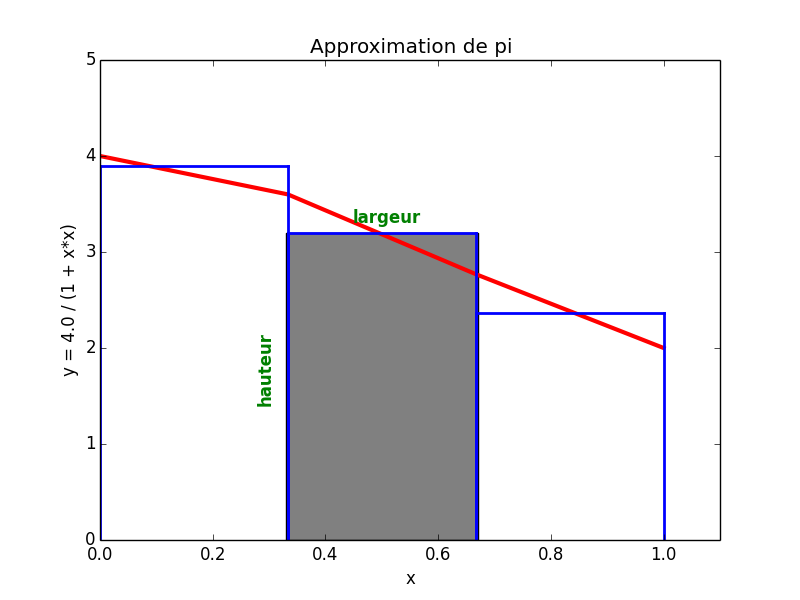
\includegraphics[height=1.8in]{images/Chapitre1/pic_pi_rect_1.png}
                    \caption{Approximation avec 4 rectangles}
                \end{subfigure}%
            \begin{subfigure}[t]{0.5\textwidth}
                    \label{pic_pi_2}
                    \centering
                    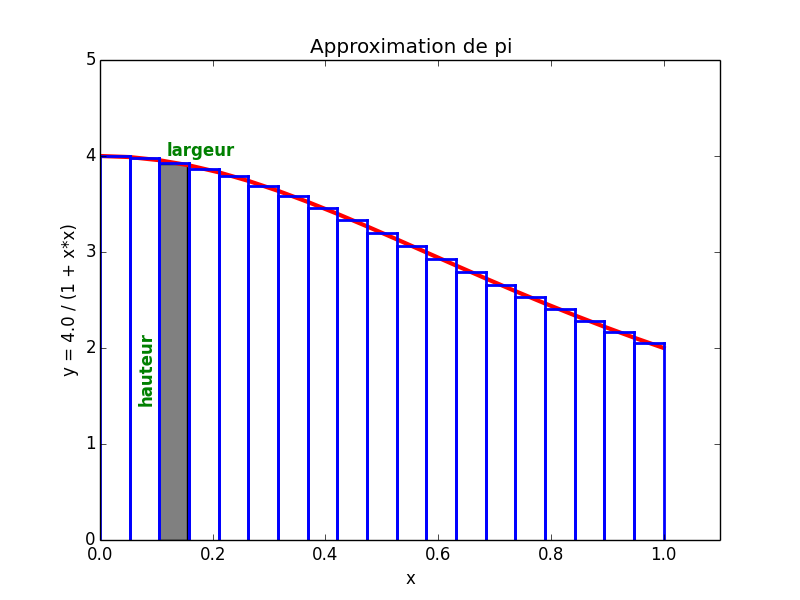
\includegraphics[height=1.8in]{images/Chapitre1/pic_pi_rect_2.png}
                    \caption{Approximation avec 14 rectangles}
                \end{subfigure}
                \caption{Méthode des rectangles: exemple de deux exécutions de l'algorithmes un nombre de rectangles différents.}
                \label{pic_pi_rect}
            \end{figure}
            
            \begin{lstlisting}[language=C, caption=Implémentions de l'algorithme de calcul d'intégrale par la méthode des rectangles, float,floatplacement=H]
double x, largeur, hauteur, pi = 0.0;

int num_steps = 4;
int num_steps = 14;

largeur = 1.0 / num_steps;

for (int i = 0; i < num_steps; ++i) {
    x =  (i) * largeur;
    hauteur = ( 4.0/(1.0+x*x));
    pi += largeur * hauteur;
}

cout << "Valeur de pi: " << pi << endl;
\end{lstlisting}
    
        Nous présentons cette exemple simpliste pour illustrer le besoin de puissance de calcul pour réaliser des simulations précises. On remarque sur la \autoref{pic_pi_1}, qu'avec l'utilisation de quatre rectangles, la surface des rectangle ne correspond pas exactement à la courbe à approximer. Ces erreurs affecte la précision de notre programme qui affiche une valeur de $\pi = 3.38$. La \autoref{pic_pi_2} présente le même programme qui utilise 14 rectangles. Les rectangles sont alors plus fidèles à la courbe et le programme calcul une valeur de $\pi = 3.21$.
        
        La précision du calcul dépend donc du nombre de rectangle choisi. Plus le nombre de rectangles utilisé est grand, plus la précision augmente. Dépendant, augmenter le nombre de rectangles à calculer augmente le nombre d'opérations nécessaires à réaliser.
        
        Les simulations numériques utilisées dans le domaine du HPC sont plus complexe que cet exemple qui n'a pour seul objectif que de montrer le liens entre puissance de calculs et précision. Lorsque le calcul à réaliser est trop complexe pour être exécuté dans un temps raisonnable, le travail à réaliser doit être partagé entre les ressources de calculs. Dans cet exemple, un ou plusieurs rectangles pourrait être assigné à chaque ressources de calculs (coeurs ou serveur) qui s'occuperait alors de calculer sa partie. À la fin de l'exécution, un dernier processeur s'occupera alors de la sommation des différents résultats. Ce travail, appelé programmation parallèle, doit être réalisé par le programmeur qui peut s'aider de librairie déjà existante ou d'un compilateur suffisamment évolué pour extraire la parallélisme de ce programme
        



 
        \subsubsection{Niveau de parallélisme des supercalculateurs}
        %%%%%%%%%%%%%%%%%%%%%%%%%%%%%%%%%%%%%%%%%%%%%%%%%%%%%%%%%%%%%%
            
            Pour obtenir les meilleurs performances d'un supercalculateur, une application doit utiliser toutes les sources de parallélisme disponibles. Ces différentes formes ont été regroupées en quatre classes appelée taxonomie de Flynn \cite{Flynn2011}. Ces classes permettent de caractériser les architectures en fonction de l'indépendance ou du partage des données et des instructions. La classe \verb=SISD= représente les architectures classiques n'exécutant qu'une instruction sur une données à la fois. 
            La classe \verb=SIMD= regroupe les architectures vectorielles exécutant une instructions sur plusieurs données à la fois (voir \autoref{sec:cpu_vectoriel}). La classe \verb|MIMD| représente des architectures exécutant plusieurs instructions sur plusieurs données à la fois. Un serveur possédant plusieurs processeurs est un exemple d'architecture \verb|MIMD|.La dernière classe d'architecture \verb|MISD| est beaucoup plus rare. Ces dernières exécutent des instructions différentes sur le même jeu de données. Le processeur ASIC présent dans les voitures connectées peuvent par exemple exécuter deux algorithmes différents pour s'assurer de la validité d'une décision à prendre. 
            
            
            
            
            \begin{figure}
            \center
            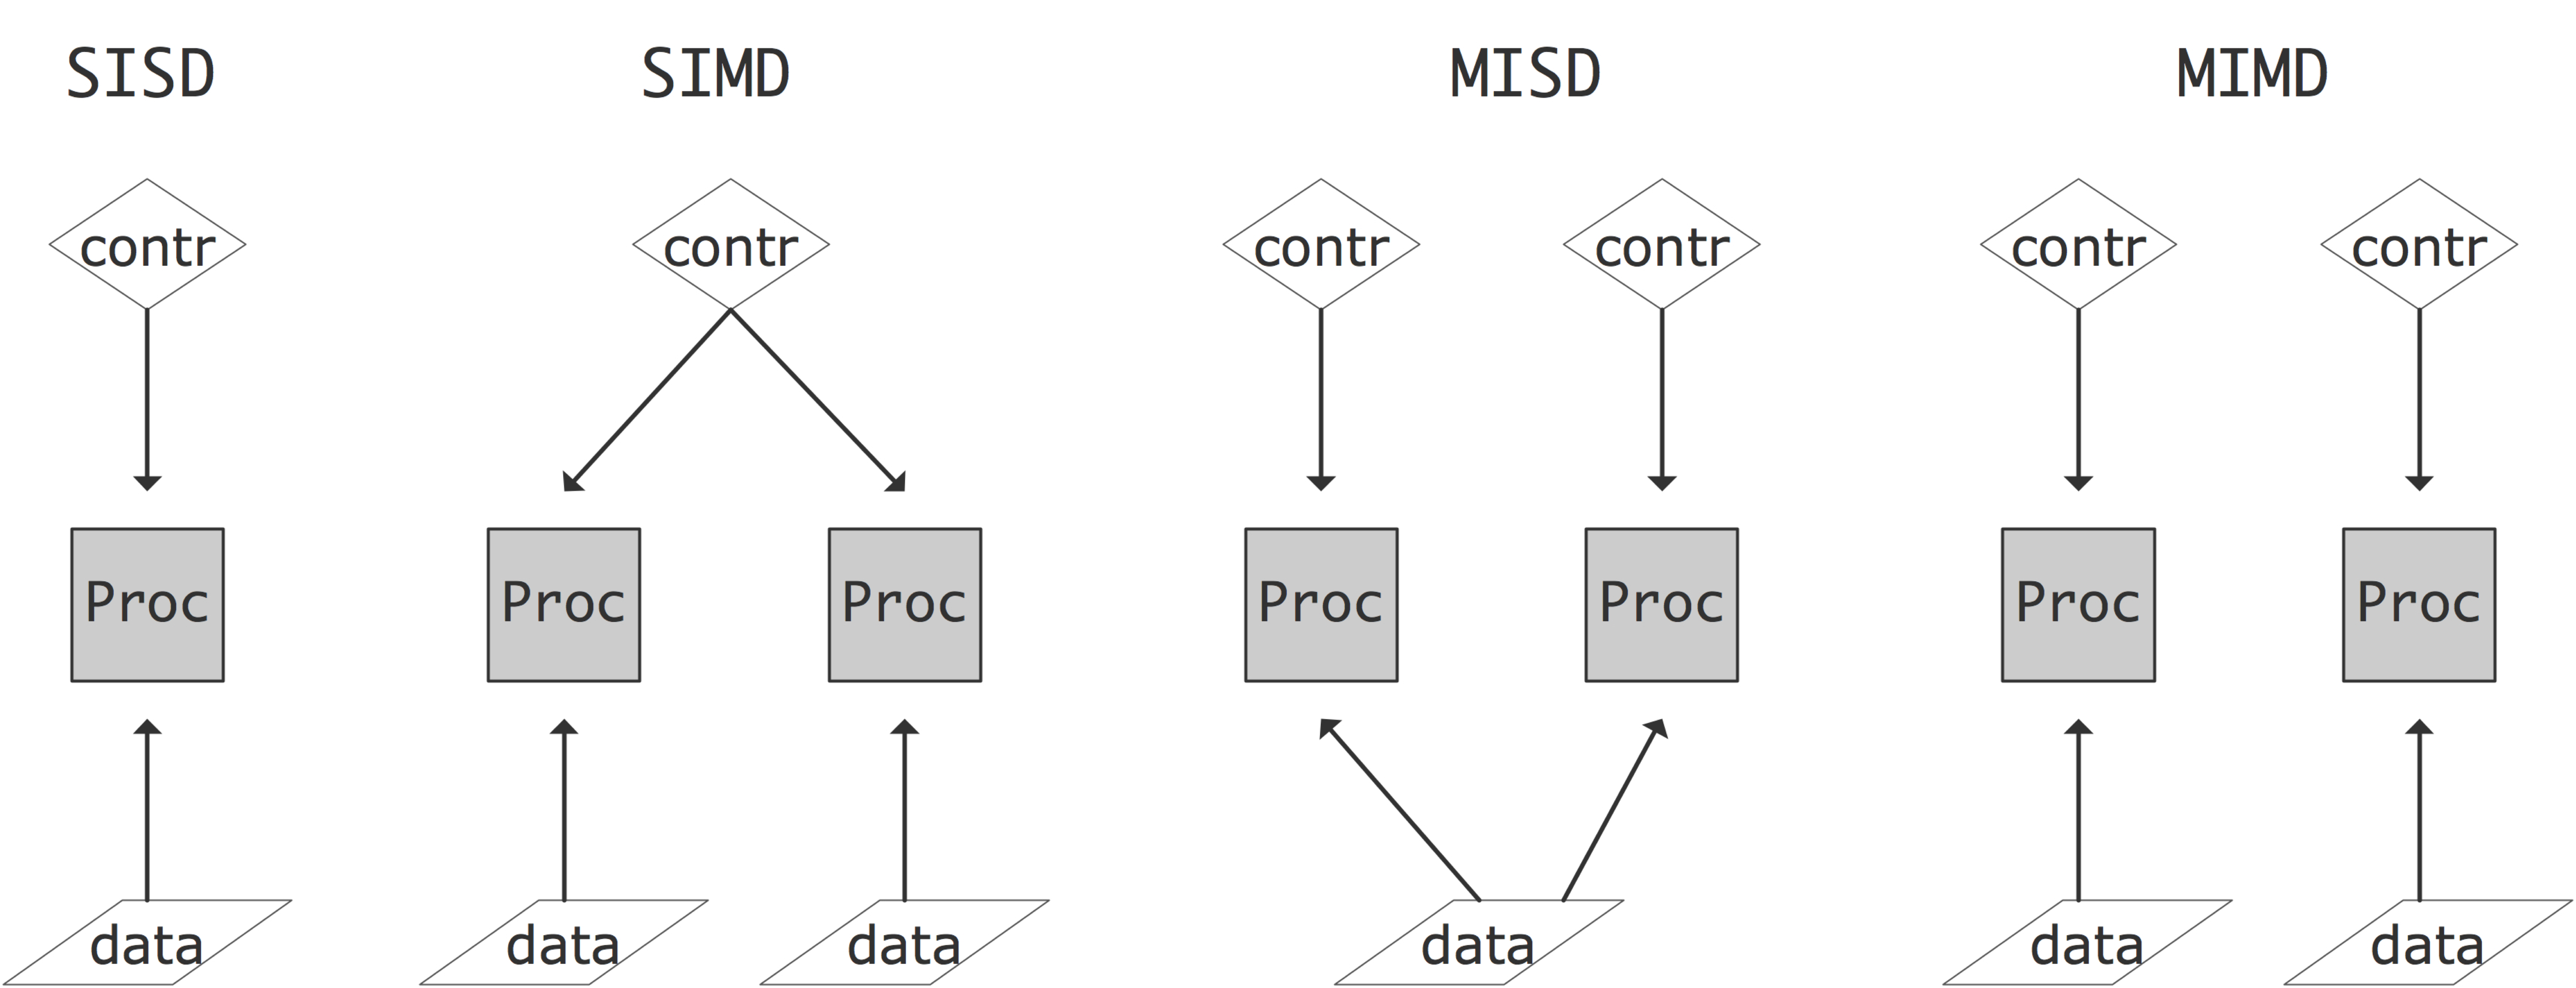
\includegraphics[width=12cm]{images/flynn.png}
            \caption{\label{fig:flynn} Les quatre classes de la taxonomie de Flynn (graphique extrait de \cite{Eijkhout2013})}
            \end{figure}
            
            
            
            
            \begin{figure}
                \center
                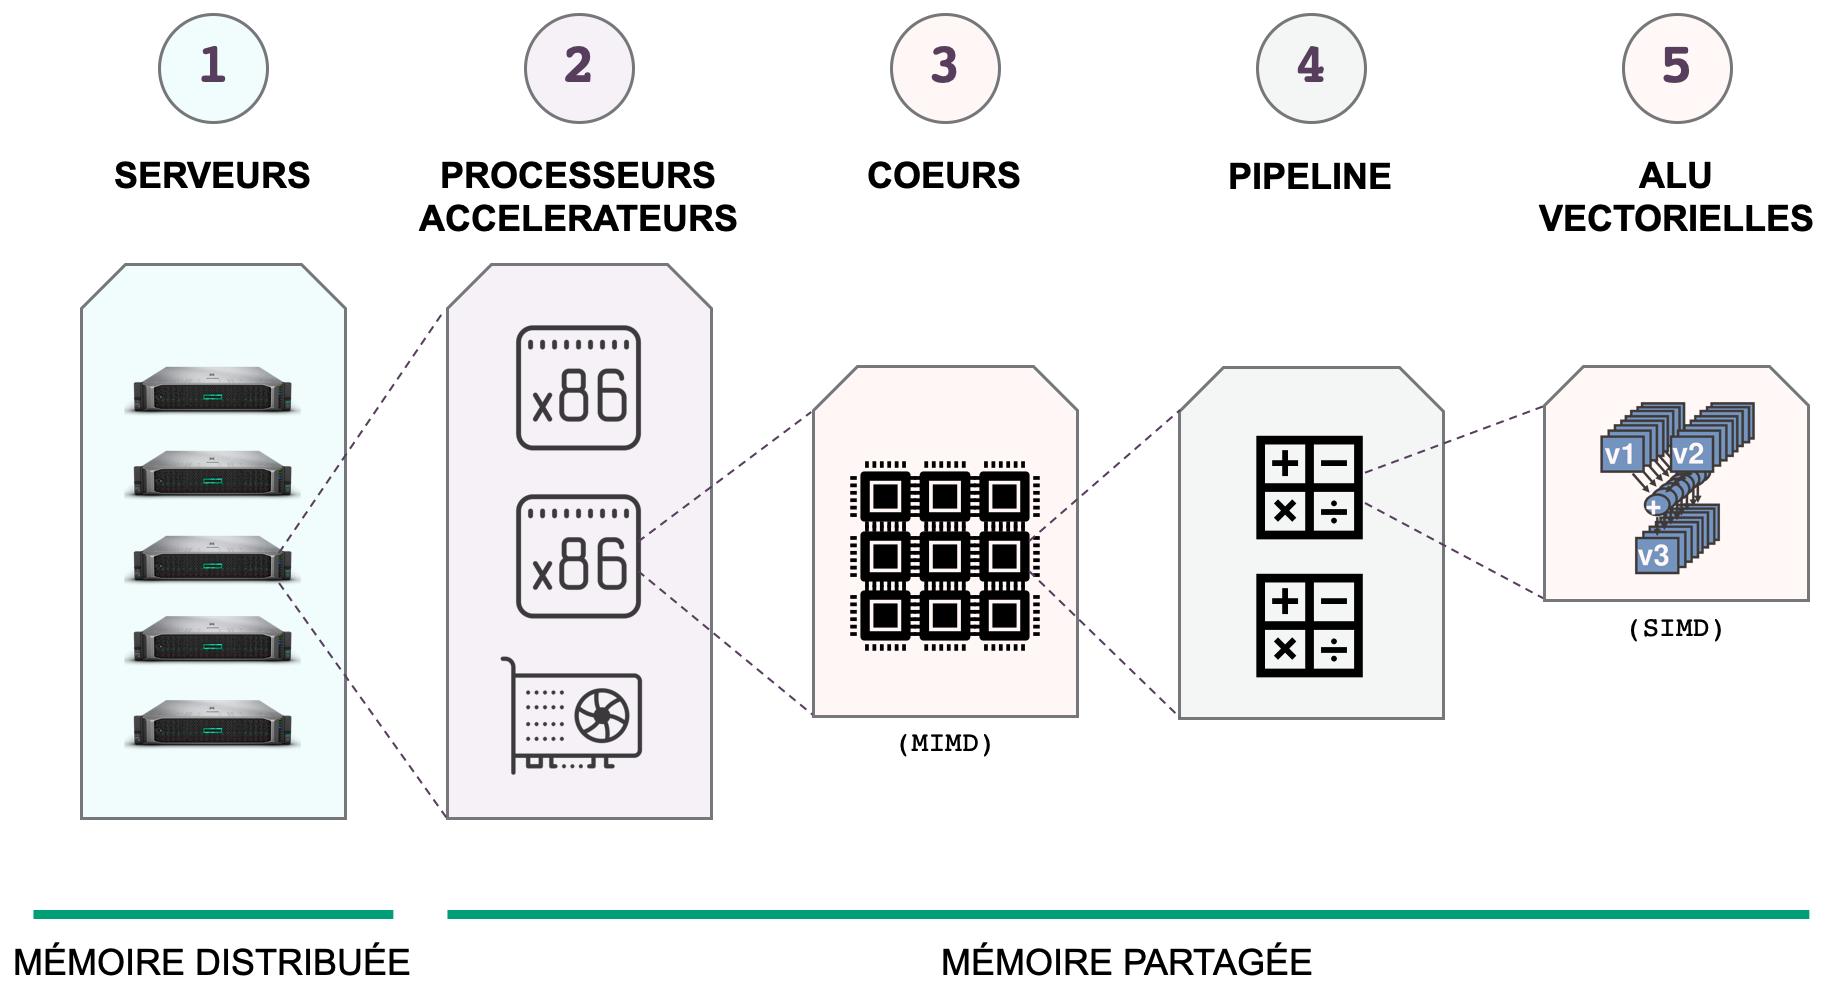
\includegraphics[width=14cm]{images/parallele_hpc.png}
                \caption{\label{fig:parallele_hpc} Différents niveaux de parallélisme dans un supercalculateur.}
            \end{figure}
    
            La \autoref{fig:parallele_hpc} représente les principaux niveaux de parallélisme d'un supercalculateur.
            Le premier niveau concerne les serveurs. Relié par un réseaux, des tâches peuvent être assignés à chaque noeuds qui peuvent communiquer entre eux pour se synchroniser ou partager des résultats. 
            Le second niveau concerne le parallélisme des processeurs (ainsi que des accélérateurs si le serveur en possède). En fonction des tâches à réaliser et des caractéristiques des ressources de calculs, les tâches peuvent être réparties pour être exécutées. 
            Le troisième niveau de parallélisme est situé dans les processeurs. Tous les processeurs utilisés dans les supercalculateurs modernes possèdent plusieurs coeurs. Ces coeurs partagent la même zone mémoire et peuvent travailler ensemble sur un même jeu de données.
            Le quatrième niveau de parallélisme est lié aux processeurs superscalaires possédant plusieurs pipeline (voir \autoref{sec:pipeline}).
            Le dernier niveau de parallélisme concerne les unité de calcul vectorielles des processeurs qui peuvent exécuter une instructions sur plusieurs données simultanément (voir \autoref{sec:fpu}).
            
            Pour maximiser le nombre d'instructions pouvant être exécutées sur un supercalculateur (\textit{Instruction Level Parallelism} (ILP)) différentes méthodes existent. Le plus haut niveau consiste à exécuter des applications indépendantes permettant de saturer l'utilisation de la plateforme (\textit{Job Level Parallelism}). Une même application peut être découpé en tâches qui peuvent être exécutées en parallèle (\textit{Task Level Parallelism} (TLP) \cite{Kambadur2009}). Lorsque la nature du code le permet, une instruction peut être exécutée sur plusieurs données simultanément (\textit{Data Level Parallelism}(DLP) \cite{Espasa1997}).
            
            
        \subsubsection{Paradigme de programmation}
        %%%%%%%%%%%%%%%%%%%%%%%%%%%%%%%%%%%%%%%%%%%%%%%%%%%%%%%%%%%%%%
       
             L'exemple du calcul de pi présenté dans la \autoref{sec:exemple_pi}, a montré que le programmeur devait modifier son code pour l'accélérer grâce au parallélisme. Deux principes fondamentaux de la programmation parallèle doivent être utilisés pour profiter des différents niveaux de parallélisation disponible dans un supercalculateur (voir \autoref{fig:parallele_hpc}).  Le choix entre les deux est à fait en fonction du mode d'accès mémoire (voir \autoref{fig:edl_ditribue_partage}). Le premier paradigme appelé programmation à mémoire partagée permet aux différents processus (\textit{threads}) de communiquer à travers l'espaces mémoire qu'ils partagent. Le deuxième paradigme appelé programmation à mémoire distribué est généralement utilisé lorsque les différents processus n'ont pas accès au même espace mémoire. Les communications sont alors réalisés par le réseau.
            
            
                        
            \begin{figure}
                \center
                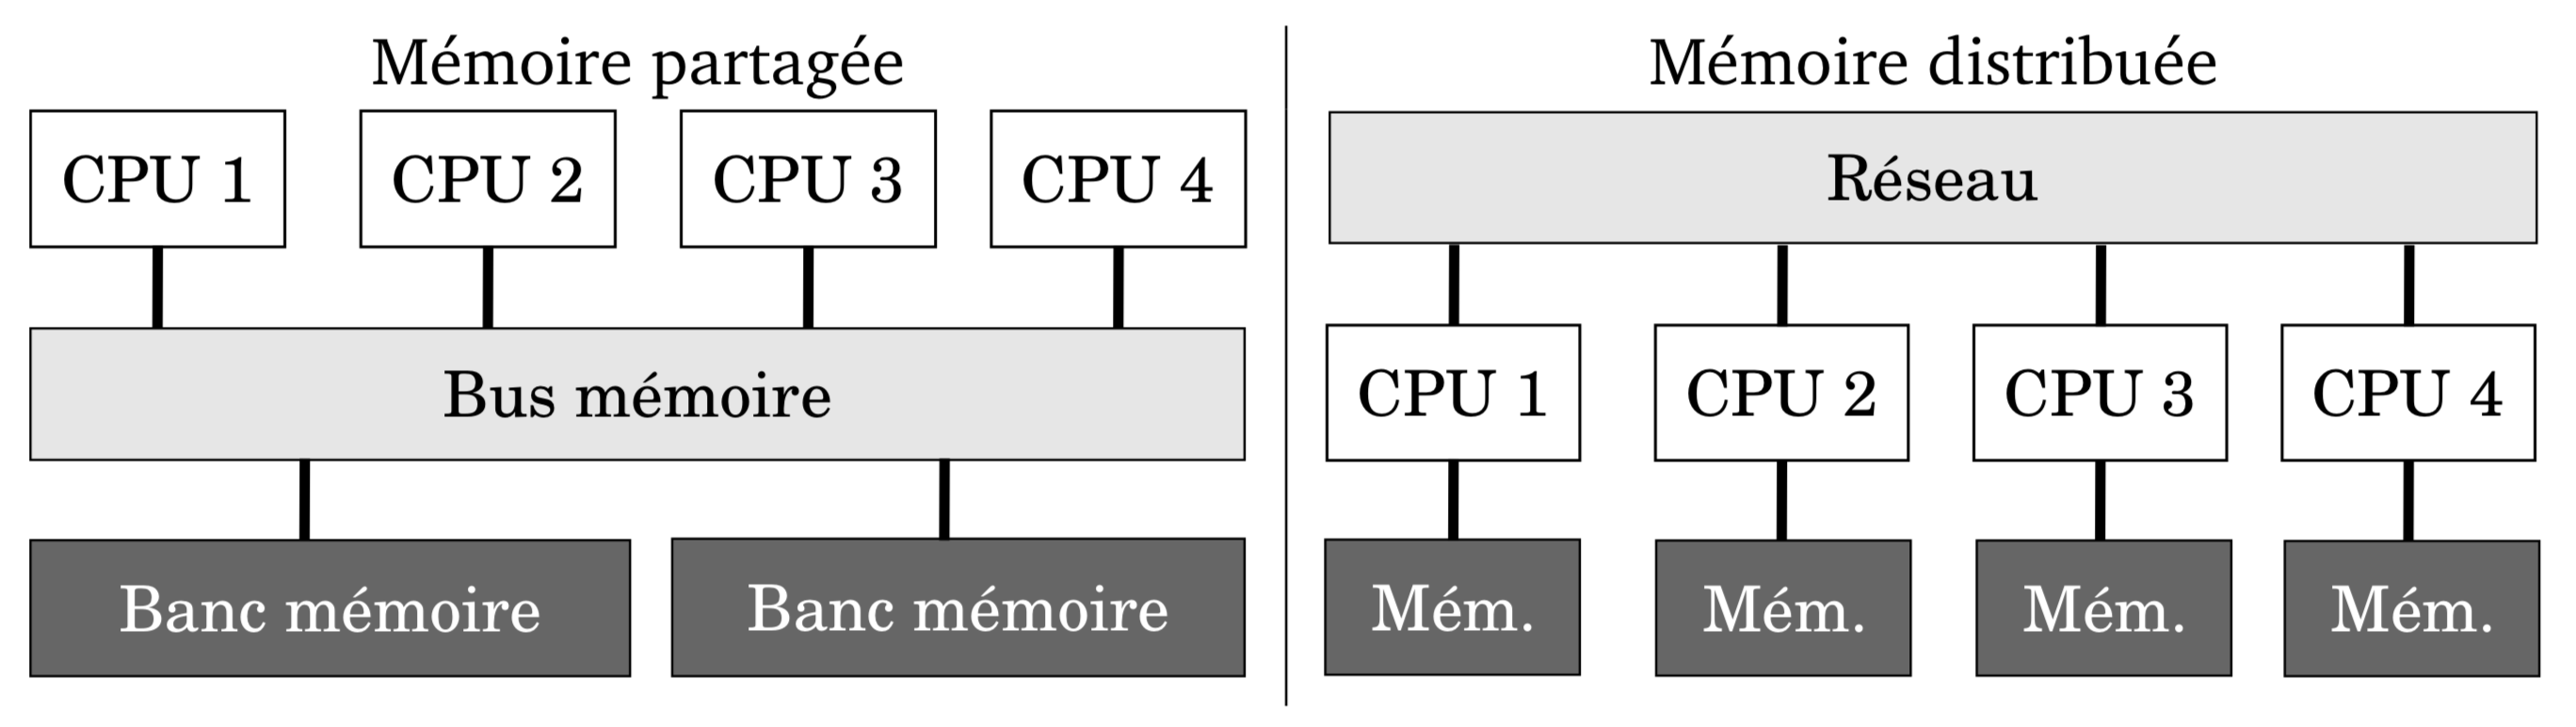
\includegraphics[width=12cm]{images/edl_ditribue_partage.png}
                \caption{\label{fig:edl_ditribue_partage} En fonction de l'architecture et du mode d'accès mémoire, deux paradigmes de programmations peuvent être utilisés (graphique etrait de \cite{Valat2016}).}
            \end{figure}
                        
            
            
            \paragraph{Programmation à mémoire distribuée.} Le premier niveau de parallélisme présenté sur la \autoref{fig:parallele_hpc} concerne les différents serveurs composant le supercalculateur. Chacun d'entre eux à son propre espace mémoire et ne peut accéder à celui des autres noeuds. Les noeuds sont reliés par un réseau d'interconnexion permettant une communication point-à-point. Pour répartir le travail sur les serveurs, l'application doit s'appuyer sur le paradigme de programmation à mémoire distribuée. Les données nécessaire pour les calculs ainsi que les résultats temporaire doivent être explicitement transférées par l'utilisateur. Le système d'interconnexion est alors capitale pour la bonne performance de ces algorithmes. Un découpage méthodique est la bonne utilisation des technique de localité est aussi nécessaire (voir \autoref{sec:locality}). 
            Le programmeur peut utiliser des librairies de \textit{passage de messages} dont le standard le plus utilisé est \verb|MPI| (\textit{message passing interface}). Le standard défini la sémantique des différentes fonctions, identifie les tâches distribuées et propose des moyens d'échanges et de synchronisation entre les processus. Le standard est implémenté par des librairies telle que \verb|OpenMPI|, \verb|MPICH-2| ou encore \verb|IntelMPI|. Chaque noeud ayant son propre système d'exploitation, les librairies doivent être installées tous les serveurs utilisés.
            La principale difficulté de ce paradigme de programmation est la nécessité de réaliser explicitement les mouvement de données entre les noeuds. La \autoref{fig:scatter_gather} présente les deux des trois phases principales d'un programme de calcul à mémoire distribué. La première étape consiste à répartir le jeu de données à l'aide d'opérations de type \textit{scatter} (voir \autoref{fig:scatter}). La deuxième étape est la réalisation du calcul par chaque ressource. Lorsque chacune d'entre elles à terminé son calcul, des opération de type \textit{gather} (voir \autoref{fig:gather}) permettent de récolter l'ensemble des résultats partiels, pour calculer le résultat final. Ces deux étapes utilisent le système d'interconnexion du supercalculateur. Les performances de celui-ci pouvant varier, les ressources peuvent alors se désynchroniser, même si un découpage parfait du jeu de données est réalisé. Cette particularité est à l'origine de nombreuses erreur et rend la programmation à mémoire distribué difficile. Le programmeur doit avoir à sa disposition des outils lui permettant de suivre l'évolution de chaque phase pour déceler des problème de synchronisation ou de déséquilibre de charge.
            
            
            \begin{figure}[t!]
                \centering
                \begin{subfigure}[t]{0.48\textwidth}
                    \centering
                    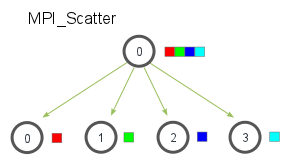
\includegraphics[width=.9\linewidth]{images/scatter.png}
                    \caption{\label{fig:scatter}Les opérations de \textit{scatter} permettent de répartir un jeu de données entre les ressources.}
                \end{subfigure}\hfill
            \begin{subfigure}[t]{0.48\textwidth}
                    \centering
                    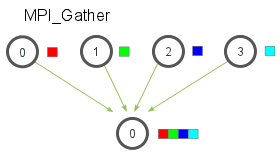
\includegraphics[width=.9\linewidth]{images/gather.png}
                    \caption{\label{fig:gather}Chaque ressources renvoi son résultat local pour calculer le résultat finale du calcul.}
                \end{subfigure}
                \caption{\label{fig:scatter_gather}Les deux opérations principales de MPI permettre de répartir et récolter les données entre les différentes ressources participant à la résolution. Le jeu de données est réparti en fonction d'un motif permettant de calculer les portions de données à envoyer.\protect\footnotemark.}
            \end{figure}
            \footnotetext{Source des graphiques - \url{https://mpitutorial.com/tutorials/mpi-scatter-gather-and-allgather/}}
           
           
           
            \paragraph{Programmation à mémoire partagée.} Lorsque toutes les ressources de calculs ont accès au même espace mémoire il est conseillé d'utiliser le paradigme de programmation à mémoire partagée. Comme il n'est plus utile de transférer les données explicitement entre les ressources de calcul, il est préférable d'utiliser des processus légers (\textit{thread}). Pour profiter des niveaux de parallélisme $2$ et $3$ (voir \autoref{fig:parallele_hpc}) le programmeur doit avoir recours à des librairies ou même des langages spécifiques aux processeurs ciblé. Les accélérateurs de type GP-GPU peuvent être programmé à l'aide d'\verb|OpenCL| ou de \verb|CUDA|. Pour les processeurs, des librairies telles que \verb|OpenMP| ou \verb|Pthread| sont utilisées pour accédées au niveau $3$ de parallélisme qui consiste à répartir l'application sur les différents coeurs. Ce librairies sont basées sur le modèle de programmation \verb|fork/join| (voir \autoref{fig:openmp}). Lorsqu'une partie du code doit être exécutée en parallèle, le thread \textit{maître} se dédouble (\textit{fork}) en plusieurs \textit{threads} pouvant être exécutés indépendament sur différent coeurs. Une fois les tâches différentes, les \textit{threads} ainsi crée sont arrêtés et le programme continue sont exécution séquentiellement. Ce modèle de programmation utilisant la même mémoire partagé, le programmeur doit veiller à l'utilisation de données en communs par les différents \textit{threads}. Un avantage d'\verb|OpenMP| est sa facilité d'utilisation pour exprimer le parallélisme depuis le code source de l'application. À l'aide de directives préprocesseur, les zones exécutables en parallèle doivent être annoté à l'aide de \verb|#pragma|. Différentes options permettent de définir combien de \textit{threads} doivent être générés, comment le travail à réaliser est partager ou encore les modes d'accès aux données (partagé, privé).
            Le code listé dans l'\autoref{lst:openmp} permet de répartir les différentes itérations d'une boucle (indépendantes) entre les \textit{threads}.
            
\begin{lstlisting}[language=C, caption=Implémentions de l'algorithme de calcul d'intégrale par la méthode des rectangles, float,floatplacement=H, label=lst:openmp]
#pragma omp parallel for
for (i=0;i<20;i++)
    a[i]=b[i] + 42;
\end{lstlisting}

            \begin{figure}
            \center
            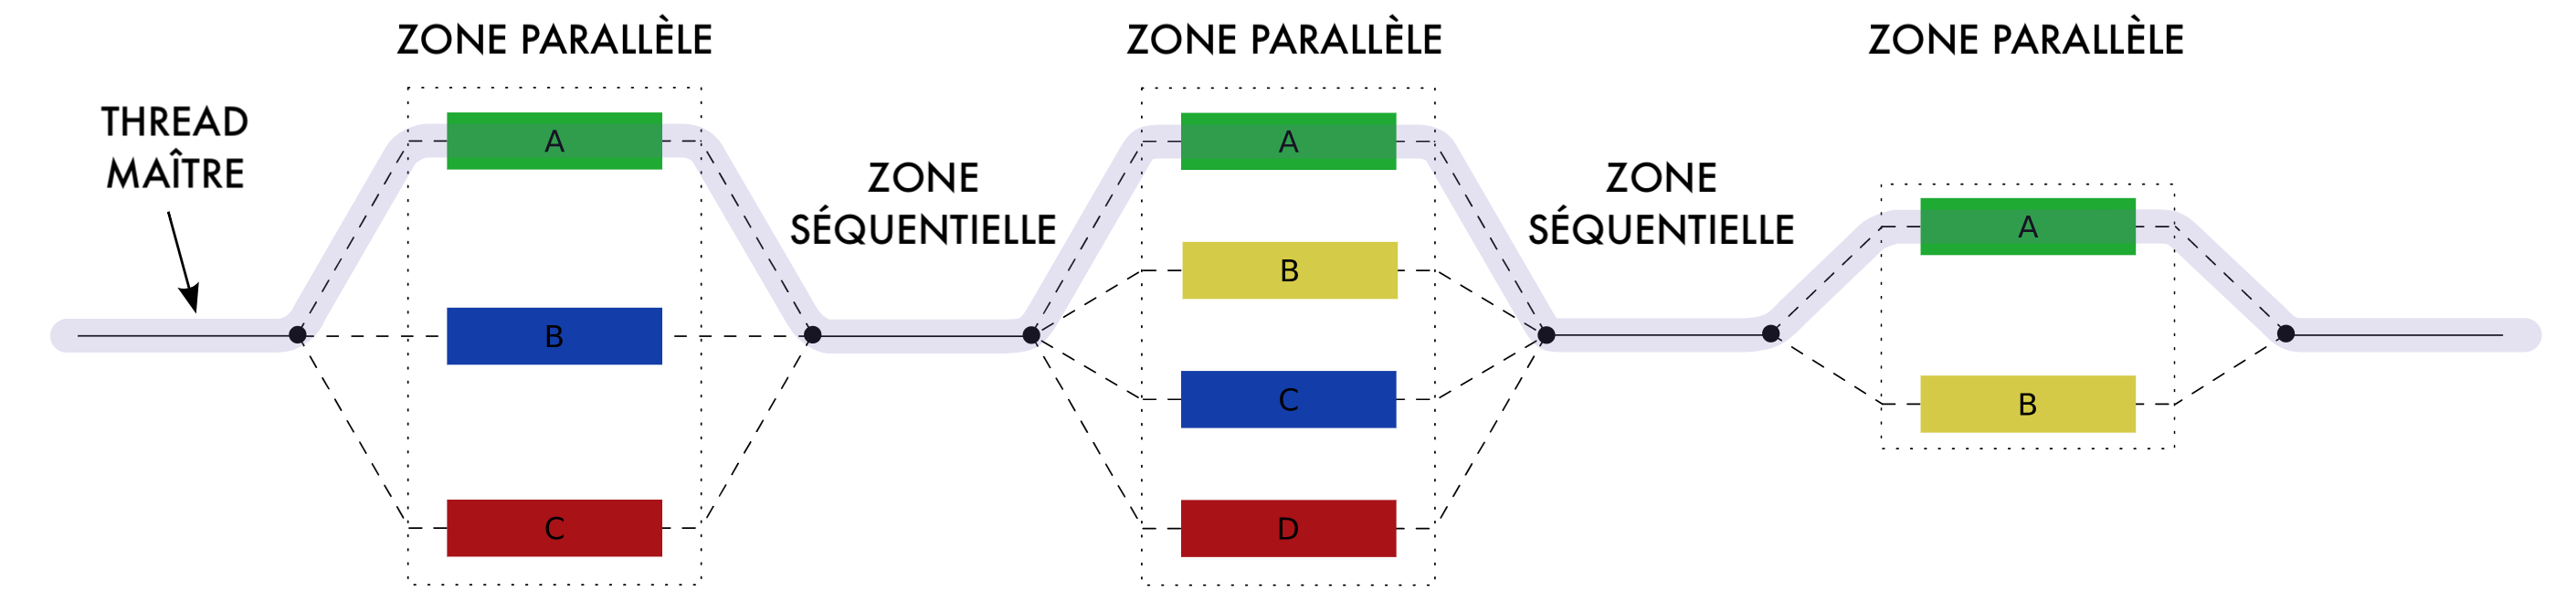
\includegraphics[width=14cm]{images/openmp.png}
            \caption{\label{fig:openmp} Pour accéder au parallélisme des coeurs, OpenMP crée des \textit{threads} indépendants\protect\footnotemark.}
            \end{figure}
            \footnotetext{Graphique adapté de \url{https://en.wikipedia.org/wiki/Fork\%E2\%80\%93join_model}}
            
            Les niveaux de parallélisme $4$ et $5$ sont géré par le matériel sans intervention du l'utilisateur. Par exemple, lorsque le compilateur génère des instructions vectorielles, l'unité de calcul s'occupe seule de leur exécution. Cependant, le programmeur doit connaître les détails de la micro-architecture pour développer du code pouvant tirer partie du parallélisme. Le module d'exécution dans le désordre (\autoref{sec:out_of_order}) permet d'optimiser l'utilisation des pipelines présents dans les processeurs superscalaires.
        
        \subsubsection{Utilisations des paradigmes dans les supercalculateurs modernes}
        %%%%%%%%%%%%%%%%%%%%%%%%%%%%%%%%
        
            Les deux paradigmes de programmations précédent possèdent tout deux leurs avantages et leurs inconvénients.
            
            La programmation à mémoire distribuée permet de construire des architectures avec de grandes ressources. Chaque serveurs ayant sa propre mémoire, au plus de serveurs sont ajoutés, au plus l'espace mémoire est grand. Chaque serveur ayant son propre espace mémoire, il n'y a pas de problèmes liés à la cohérence des caches. Un autre avantage de l'agrégation de matériels, est la possibilité d'utiliser du matériel de série (\textit{commodity hardware}). Leur coût étant moins élevé que celui d'architectures plus complexes. La performance de la solution est alors dépendante du nombre de serveurs utilisés et permet une plus grande flexibilité lors de l'achat. La programmation à mémoire distribué apporte cependant une difficulté pour les programmeurs. Les applications doivent être modifiée et utiliser des librairies supplémentaire (\verb|MPI|). Les échanges de données et la synchronisation doivent être réalisé explicitement par l'application, pouvant donné lieu à des erreurs ou à de mauvaises performances (mauvaises synchronisation, mauvaise répartition des tâches).
            
            La programmation à mémoire partagée permet au différents processus (ou \textit{thread}) d'une application de partager le même espace mémoire. La majorité des communications étant implicites (réalisées à travers des structures de données partagées), la programmation en est facilité. Ceci facilite grandement la programmation et permet d'obtenir de meilleurs performances en partageant un même jeu de données entre plusieurs processus. Le matériel est alors capable de gérer la cohérence des caches entre les différents coeurs. Cependant cette faculté à gérer la cohérence implique l'utilisation d'architectures plus complexes et ne permet pas une bonne scalabilité au delà de quelques dizaines de noeuds. 
            
            Pour allier les avantages des deux paradigmes, les supercalculateurs modernes utilisent les deux. Cependant, la programmation de tels architectures est difficile car elle doit utiliser des librairies de calculs à mémoire distribué puis ensuite répartir le travail sur un serveur à l'aide de librairie de programmation à mémoire partagée.



\subsection{Performance de la parallélisation}\label{sec:parallele_perf}
%%%%%%%%%%%%%%%%%%%%%%%%%%%%%%%%%%%%%%%%%%%%%%%%%%%%%%%%%%
    
    Pour évaluer la capacité d'une plateforme à utiliser efficacement les ressources supplémentaires pour l'exécution d'une application, il est courant de mesurer sa scalabilité. La scalabilité d'une application est un indicateur permettant d'évaluer sa capacité de \textit{passer à l'échelle}, c'est à dire d'évaluer l'accélération de son exécution lorsque des ressources de calculs supplémentaire sont allouées. On distingue alors deux scalabilités: la forte et la faible.
    
    \paragraph{Scalabilité forte.} La complexité du problème reste constante et n'évolue pas avec le nombre de ressources de calculs supplémentaires. La taille du problème étant fixe, chaque unité de calculs a donc moins de travail à réaliser. Idéalement, le temps d'exécution doit être réduit d'un facteur $1/P$ lorsque $P$ ressources sont ajoutées (voir \autoref{fig:scaling_amdahl}). 
    
    \paragraph{Scalabilité faible.} La taille du problème évolue à mesure que des ressources supplémentaire sont alloué. Dans ce cas la, la taille du problème pour chaque unité de calcul est fixe. Dans l'idéal, le temps d'exécution de l'application doit rester constant lors de l'ajout de ressources de calculs (voir \autoref{fig:scaling_gustafson}). 
        
        \begin{figure}[t!]
            \centering
            \begin{subfigure}[t]{0.48\textwidth}
                \centering
                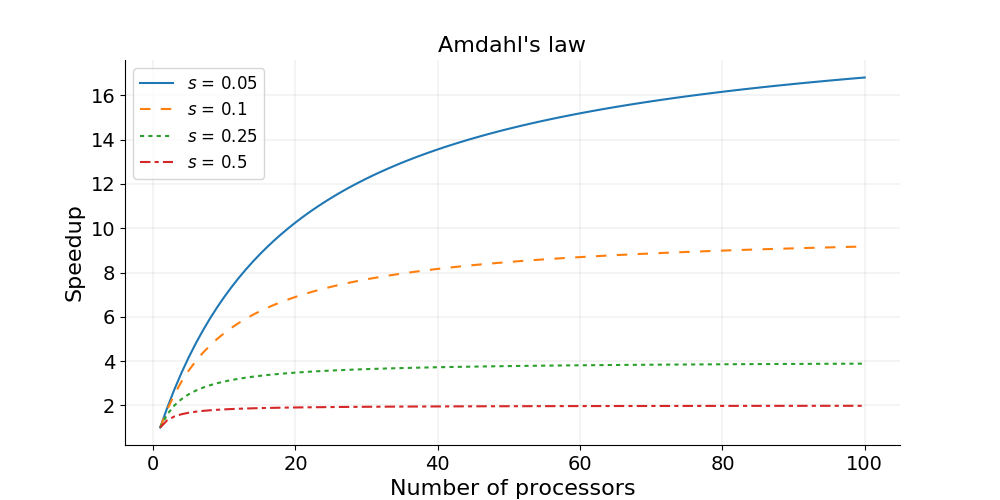
\includegraphics[width=1.05\linewidth]{images/scaling_amdahl.png}
                \caption{\label{fig:scaling_amdahl}Loi d'Amdahl: la scalabilité forte utilise un problème de complexité constante.}
            \end{subfigure}\hfill
        \begin{subfigure}[t]{0.48\textwidth}
                \centering
                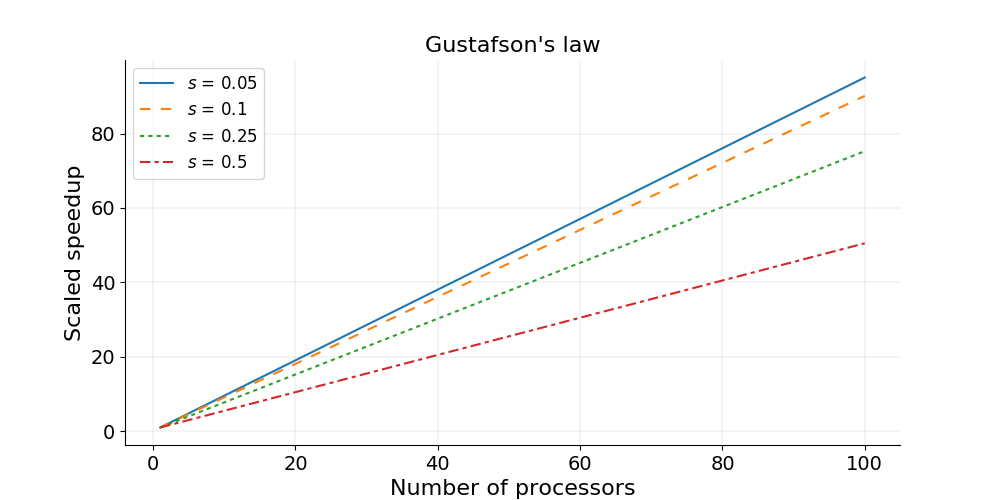
\includegraphics[width=1.05\linewidth]{images/scaling_gustafson.png}
                \caption{\label{fig:scaling_gustafson}Loi de Gustafson: la scalabilité faible utilise un problème de complexité croissante.}
            \end{subfigure}
            \caption{\label{fig:scaling}Représentation des deux types de scalabilité en fonction de la proportion de code séquentiel $s$\protect\footnotemark.}
        \end{figure}
        \footnotetext{Source des graphiques - \url{https://www.kth.se/blogs/pdc/2018/11/scalability-strong-and-weak-scaling}}
            

    \subsubsection{Accélération d'une application}
    %%%%%%%%%%%%%%%%%%%%%%%%%%%%%%%%%%%%%%%%%%%%%%
    
        L'utilisation d'un supercalculateur à pour objectif d'accélérer l'exécution d'une application. Cette accélération peut alors permettre d'obtenir des résultats plus rapidement ou bien d'étudier des problèmes plus complexes. L'accélération $Speedup$ d'une application correspond au rapport entre le temps nécessaire pour l'exécuter l'application sur une ressource ($T_{sequentiel}$) et le temps obtenu lors de l'éxécution parallèle ($T_{parallele}$):
        
        \begin{equation}
        \label{eq_speedup}
        Speedup = \frac{T_{sequentiel}}{T_{parallele}}
        \end{equation}
        
        L'accélération optimale d'une application évolue linéairement avec le nombre $P$ de ressources, le travail étant alors partagé équitablement. On parle alors d'accélération linéaire:
        
        \begin{equation}
        Speedup_{lineaire} (P) = \frac{T_{sequentiel}}{T_{parallele}} = P
        \end{equation}
            
        En pratique il est très rare d'obtenir une telle accélération car certaines partie du code ne peuvent pas être parallélisé (transmission des données en programmation à mémoire distribuée, zone critique en programmation à mémoire partagée). De plus, l'utilisation de la programmation parallèle apporte des côuts supplémentaire (notés $T_{couts}$) liés aux communications des données et à la synchronisation des processus.
        \begin{equation}
        T_{parallele} = \frac{T_{sequentiel}}{P} + T_{couts}
        \end{equation}
  
    
  
    \subsubsection{La loi d'Amdahl} 
    %%%%%%%%%%%%%%%%%%%%%%%%%%%%%%%%%%
        
        
        En 1967, l'ingénieur Gene Amdahl a étudié et théorisé l'évolution de l'accélération d'une application avec l'ajout de ressources de calculs a été qui a donné lieu à la loi éponyme. La loi d'Amdahl permet de donner la limite théorique de l'accélération $Speedup$ d'une application lorsque des ressources de calculs supplémentaires sont utilisées pour la résolution d'un problème de taille fixe. Une application de calcul parallèle n'est jamais totalement parallélisable. Elle possède toujours certaines zones de code, notées $s$, devant être exécutées séquentiellement. L'ajout de ressources de calculs n'est alors bénéfique que pour les zones parallèles, notée $1-s$. Le temps nécessaire pour l'exécution de l'application est la somme du temps passé dans la zone séquentielle et de celui passé dans la zone parallèle. En supposant des coût $T_{couts}$ associés à l'utilisation du parralélisme, le temps d'exécution du programme parallélisé peut être calculé ainsi : 
        \begin{equation}
        T_{parallele} = s \times T_{sequentiel} + \frac{(1-s) \times T_{sequentiel}}{P}
        \end{equation}
        
        
        L'accélération de l'application peut alors être calculé grâce à l'\autoref{eq_speedup} donnant lieu à l'équation suivante, appelée Loi de Amdahl:
        
                
        \begin{equation}
        \label{eq_amdahl}
        Speedup (P) = \frac{T_{sequentiel}}{s \times T_{sequentiel} + \frac{(1-s) \times T_{sequentiel}}{P}} =  \frac{1}{s + \frac{1-s}{P}}
        \end{equation}
        
        L'accélération d'une application dépend donc du nombre de ressources de calculs supplémentaires allouées à la résolution de l'application mais aussi de la proportion de zone exécutable en parallèle. La \autoref{fig:scaling_amdahl} montre combien la proportion $1-s$ de code parallélisable influe sur l'accélération de l'application. 
  
        La loi d'Amdahl permet par exemple de connaître l'accélération maximale ($Speedup_{max}$) d'une application passant 95\% de son temps d'exécution dans une fonction entièrement parallélisable. Cette accélération peut être calculé par la limite suivante:
        \begin{equation}
        Speedup_{max} =  \lim_{p\to\infty}    \frac{1}{0.05 + \frac{0.95}{P}} = \frac{1}{0.05} = 20
        \end{equation}
        Quel que soit le nombre de ressources allouées à l'exécution de cette application, l'application étudiée en exemple ne pourra jamais être accéléré de plus de 20 fois.  
       

    
    \subsubsection{Loi de Gustafson} 
    %%%%%%%%%%%%%%%%%%%%%%%%%%%%%%%%%%
        
        La loi d'Amdahl est très utile pour montrer la nécessité de développer des applications avec la plus grande portion de code parallélisable. Cependant, la loi suppose une taille de problème constante. Lorsque des ressources de calculs supplémentaire sont disponibles, les applications utilisent généralement des jeux de données plus grand pour profiter de l'espace mémoire supplémentaire. La loi d'Amdahl supposant un jeu de donnée fixe, ne s'applique alors plus. Pour y remédier, Gustafson énonça une nouvelle loi en 1988 \cite{Gustafson1988} permettant de prendre cet aspect en considération.  Lorsque que la taille du jeu de données augmente, la partie séquentielle du programme représente généralement une plus faible portion car les données sont traitées dans les zones parallèles. L'accélération peut alors être calculé par la formule suivante, appelée loi de Gustafson:
        \begin{equation}
        Speedup (P) = s + (1-s) * P
        \end{equation}
        
        
        













